\chapter{ML for Mathematics}
\label{ch:08-ml-for-mathematics}

\lecturemeta{Matija Tapu\v{s}kovi\'{c}}{University of Oxford}

Tapu\v{s}kovi\'{c} is a mathematician rather than a machine learning researcher, and the talk
asks one question: can machine learning discover new mathematics? The answer is organised into
three strands, learning from examples, searching in language space, and formalisation, and the
recurring test applied to each is the one a mathematician would apply: where does the machine's
output re-enter mathematics? Not whether a metric improved, but whether the result becomes a
theorem, a conjecture someone will chase, or merely a number. The conclusion running through all
three strands is that the search is rarely the bottleneck. Building a cheap, exact and
ungameable evaluator is the research.

\section*{Key ideas}

\paragraph{Strand I, learning from examples, works when attribution is interpretable.} The
flagship result is on Kazhdan--Lusztig polynomials. A permutation becomes a directed graph, an
interval $[x,y]$ in the Bruhat order becomes a subgraph, and the combinatorial invariance
conjecture of Lusztig and Dyer says isomorphic unlabelled interval graphs give the same
polynomial. A message-passing GNN was trained on the bare interval graph to predict the
coefficients of $P_{x,y}$, and gradient attribution flagged particular edges as
overrepresented~\citep{davies2021}. Those flagged edges pointed at a decomposition: a recipe
computes $P_{x,y}$ from a split of the interval into two smaller pieces, though the recipe needs
labels, and the new conjecture is that any valid split agrees, which would imply combinatorial
invariance (Figure~\ref{fig:ml-for-mathematics-1}). A variant of that conjecture has since been
proved for broad families. The point is that the network's value was not its accuracy but the
fact that its attribution was legible enough to become a mathematical statement.

\begin{figure}[htbp]
\centering
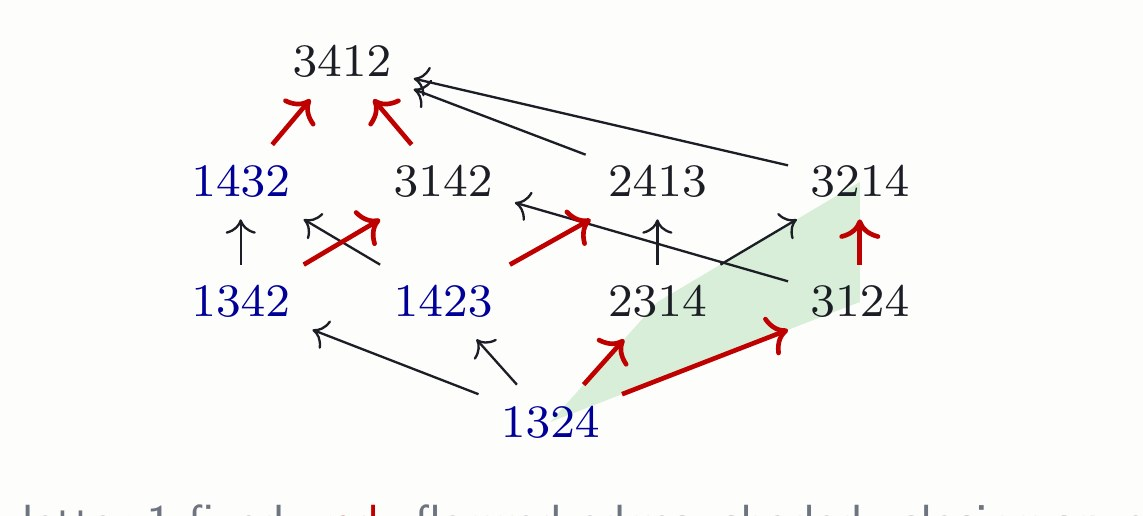
\includegraphics[width=0.68\textwidth]{figures/ml-for-mathematics-1.jpg}
\caption{The output that re-entered mathematics, from the ML for Mathematics lecture. An
interval in the Bruhat order on permutations, drawn as a directed graph. Red marks the edges
that gradient attribution on the trained GNN flagged as overrepresented, blue marks vertices
whose first letter is fixed, and the shaded region is the closing square of the split those
flagged edges suggested. This picture, not the model's accuracy, is what became a conjecture.}
\label{fig:ml-for-mathematics-1}
\end{figure}

\paragraph{The counterexample in the same strand is instructive.} On elliptic curves
$E: y^2 = x^3 + Ax + B$, the rank in
$E(\mathbb{Q}) \cong E(\mathbb{Q})_{\text{tors}} \oplus \Z^{\rank(E)}$ is not directly
computable, so the experiment represented each curve by its sequence of point counts
$a_p = (p+1) - N_p(E)$ and ran logistic regression on $(a_2, a_3, \dots) \in \Z^{500}$ to
separate rank 0 from rank 1, reaching over 97\% accuracy and beating known
heuristics~\citep{he2022}. The expert reaction quoted on the slide is the lesson: what has been
learned is the sign in the functional equation of the associated $L$-function, not the rank. The
model was right for a reason that made it uninformative, and the data came from an archive
rather than a generator, which limits what could be probed.

\paragraph{A worked case study in why data, not method, is the constraint.} The Feynman-integral
material is the most detailed part of the lecture and reads as a cautionary tale told against
the speaker's own field. The question is whether weight drop, conjecturally equivalent to
$c_2 = 0$, is visible in elementary graph features. On 1,958 graphs up to 11 loops with 272
positives and 24 features, AUC was 0.90. Then the deflation begins. The top feature restates a
known theorem, that a 3-vertex cut forces a product and hence $c_2 = 0$; remove those positives
and AUC falls to 0.85. The 165 survivors form only 7 families with labels constant within a
family, so the classifier is largely recognising disguised siblings; hold out whole families and
AUC falls to 0.74. In the full catalogue of 283 irreducible families up to 10 loops, exactly 7
have the drop, and those 7 are conspicuous anyway, with automorphism groups roughly twenty times
larger than typical and degenerate, often integer, spectra. With 7 positives the finding is a
description, not a rule. Two further constraints are named: labels are genuinely expensive, since
at 11 loops $c_2$ is known at only four primes and the next prime can cost hours per graph; and
GNNs are the wrong tool here because $\phi^4$ graphs are 4-regular, so a message-passing network
is blind by 1-WL to exactly the signal that works, which points at the geometric deep learning
toolkit as the fix (Chapter~\ref{ch:11-geometric-deep-learning}).

\paragraph{Strand II, search in language space, when there is no dataset.} The reframing is that
a scoring function is enough to enable search, and the key move is not to search the space of
objects but the
space of programs that generate them, so that a program inherits the score of its output and an
LLM proposes variants. The lineage given runs from extremal-combinatorics search through
PatternBoost to FunSearch and AlphaEvolve. The flagship evaluation is 67 problems, hours each,
almost all of the form improve a bound on a constant, with a scorecard of 20 new, 39 matched and
8 fell short~\citep{georgiev2025}. The authors' own framing is quoted rather than softened: none
of the results is individually important, every one could have been found with standard tools, and
the point is time; the tool beats the literature where the literature is thin and matches or
trails it where it is deep. The concrete highlight is Kakeya and Nikodym sets over finite fields,
where the previous Kakeya record in dimension three was
$\tfrac14 p^3 + \tfrac78 p^2 + O(p)$ and AlphaEvolve found
$\tfrac14 p^3 + \tfrac78 p^2 - \tfrac18$ for $q = p \equiv 1 \bmod 4$, a two-line formula over
quadratic residues. For Nikodym sets the machine's idea, delete surfaces rather than points, was
no better than random as used, and a human repaired it by hand into a genuine improvement. The
recurring observation is that the expertise moved into the evaluator.

\paragraph{Strand III, certainty.} A proof assistant checks that a term inhabits a type, so
compiling a statement establishes well-formedness, not truth, and the proof term is what must be
constructed. The motivating question is sharp: would any expert read a 150-page proof of a major
conjecture handed over by a language model? Formal infrastructure is
uneven, with mathlib at roughly 2.3M lines built over nine years, covering approximately an
undergraduate degree and jagged beyond it. The competition trajectory given is 2024 AlphaProof
and AlphaGeometry at silver with the kernel as evaluator, 2025 Deep Think at gold in plain
English graded by humans, and 2026 AxiomProver at 42 out of 42, formal end to end, roughly 8,000
lines of Lean in about 25 hours. The research-level example
closes the loop: for minimal Kakeya sets in $\mathbb{F}_p^3$, AlphaEvolve found the construction,
Deep Think proved it and AlphaProof certified it, the full pipeline closed, but only because every
ingredient was already in mathlib. In dimension 4 elliptic curves appear and the certification
fails; for Nikodym sets the construction was too tangled to analyse and the final proof was
entirely human. The frontier of machine certification runs out precisely where the deep objects
begin.

\section*{Notation}

$S_n$ is the symmetric group, $P_{x,y}(q)$ a Kazhdan--Lusztig polynomial, $E$ an elliptic curve
with $a_p$ its trace of Frobenius at $p$, $c_2$ the Feynman-graph invariant whose vanishing is
weight drop, and $\pi(x)$ the prime counting function.

\section*{Why it matters}

This chapter is a rigorous account of what it takes for a machine learning result to count as a
contribution in a field with an external standard of correctness, which makes it the sharpest
methodological lecture of the week. Its central complaint, that the evaluator is the research and
the search is not the bottleneck, transfers directly to reinforcement learning
(Chapter~\ref{ch:04-intro-reinforcement-learning}), where RLVR is exactly the claim that a
cheap, exact, ungameable reward changes what is learnable. The Feynman-graph observation that
4-regularity makes message passing blind is a concrete instance of the expressivity limits that
Chapter~\ref{ch:11-geometric-deep-learning} addresses by construction.

\begin{aside}
The three strands are an escalating standard of evidence, and the same ladder can be applied to
ordinary machine learning work. Strand I asks whether a model's attribution
is legible enough to state as a claim. Strand II asks whether the score is faithful enough that
optimising it means something. Strand III asks whether the result can be checked without trusting
the producer. Most machine learning papers only clear the second bar, and clear it against a
metric far less exact than a Lean kernel.
\end{aside}
